\documentclass{standalone}
\usepackage{pgfplots}
\pgfplotsset{compat=1.18}
\usepgfplotslibrary{colorbrewer}
\pgfplotsset{cycle list/Set1-6}

\begin{document}

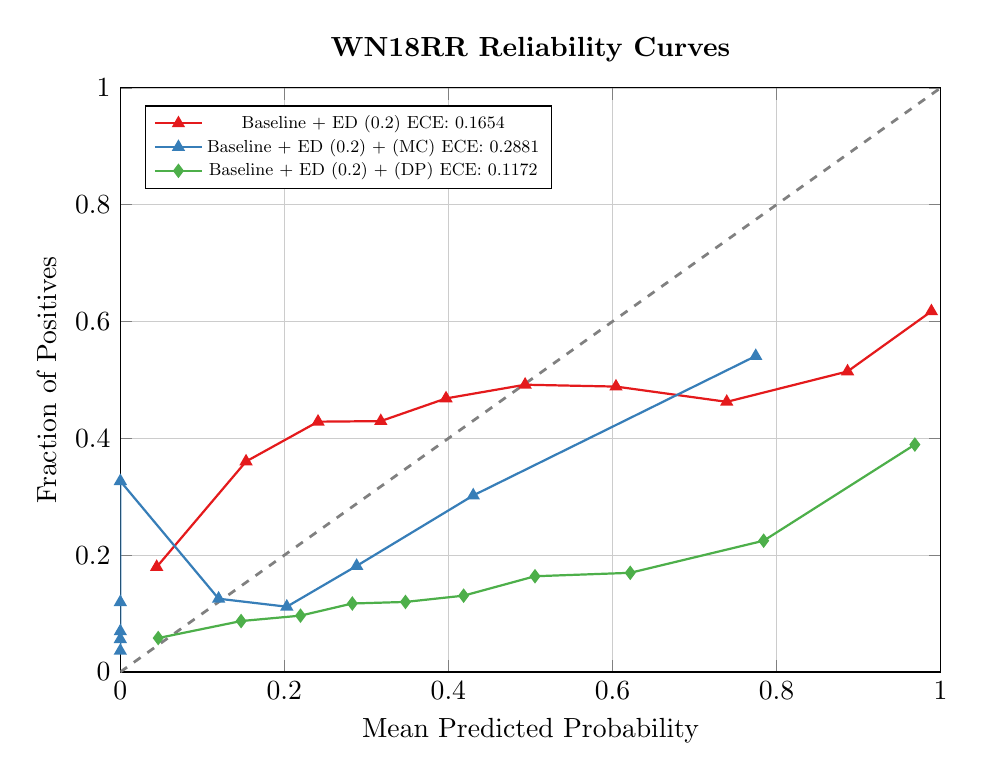
\begin{tikzpicture}
\begin{axis}[
    title={\textbf{WN18RR Reliability Curves}},
    xlabel={Mean Predicted Probability},
    ylabel={Fraction of Positives},
    xmin=0, xmax=1,
    ymin=0, ymax=1,
    xtick={0, 0.2, 0.4, 0.6, 0.8, 1.0},
    ytick={0, 0.2, 0.4, 0.6, 0.8, 1.0},
    legend pos=north west,
    legend style={nodes={scale=0.7, transform shape}, font=\small},
    grid=both,
    grid style={line width=.1pt, draw=gray!20},
    major grid style={line width=.2pt, draw=gray!40},
    width=12cm,
    height=9cm,
    cycle list name=Set1-6
]

% Perfectly Calibrated Line
\addplot [color=gray, dashed, line width=1pt, forget plot]
    coordinates {(0,0)(1,1)};

% Baseline + Edge Dropout (0.2) + Label Smoothing (0.1)
\addplot+[mark=triangle*, thick] coordinates {
    (0.04440312, 0.17977528) (0.15332931, 0.36037137) (0.24107382, 0.42853653) (0.31759054, 0.4295138) 
    (0.39709684, 0.46836062) (0.49352566, 0.49181529) (0.60428001, 0.48863914) (0.73930518, 0.46249695) 
    (0.88656463, 0.51453701) (0.98876591, 0.61748901)
};
\addlegendentry{Baseline + ED (0.2) ECE: 0.1654}

\addplot+[mark=triangle*, thick] coordinates {
    (7.68858337e-05, 0.03621329) (8.26007188e-05, 0.05617337) (8.84877887e-05, 0.06957514) (9.82695268e-05, 0.11947534)
    (1.39020184e-04, 0.32677502) (1.19910145e-01, 0.12546336) (2.03012596e-01, 0.11177645) (2.88146579e-01, 0.18163673)
    (4.30272968e-01, 0.30225264) (7.74643242e-01, 0.54091816)
};
\addlegendentry{Baseline + ED (0.2) + (MC) ECE: 0.2881}

\addplot+[mark=diamond*, thick] coordinates {
    (0.04625737, 0.05813385) (0.14731774, 0.08722209) (0.21971495, 0.09650623) (0.28285926, 0.11727339)
    (0.34768092, 0.11996091) (0.41855987, 0.13071097) (0.50555681, 0.16393843) (0.62166645, 0.1698021)
    (0.78429812, 0.224774) (0.9686335, 0.38935027)
};
\addlegendentry{Baseline + ED (0.2) + (DP) ECE: 0.1172}


\end{axis}
\end{tikzpicture}

\end{document}